

\begin{figure*}[ht!]
	\centering
	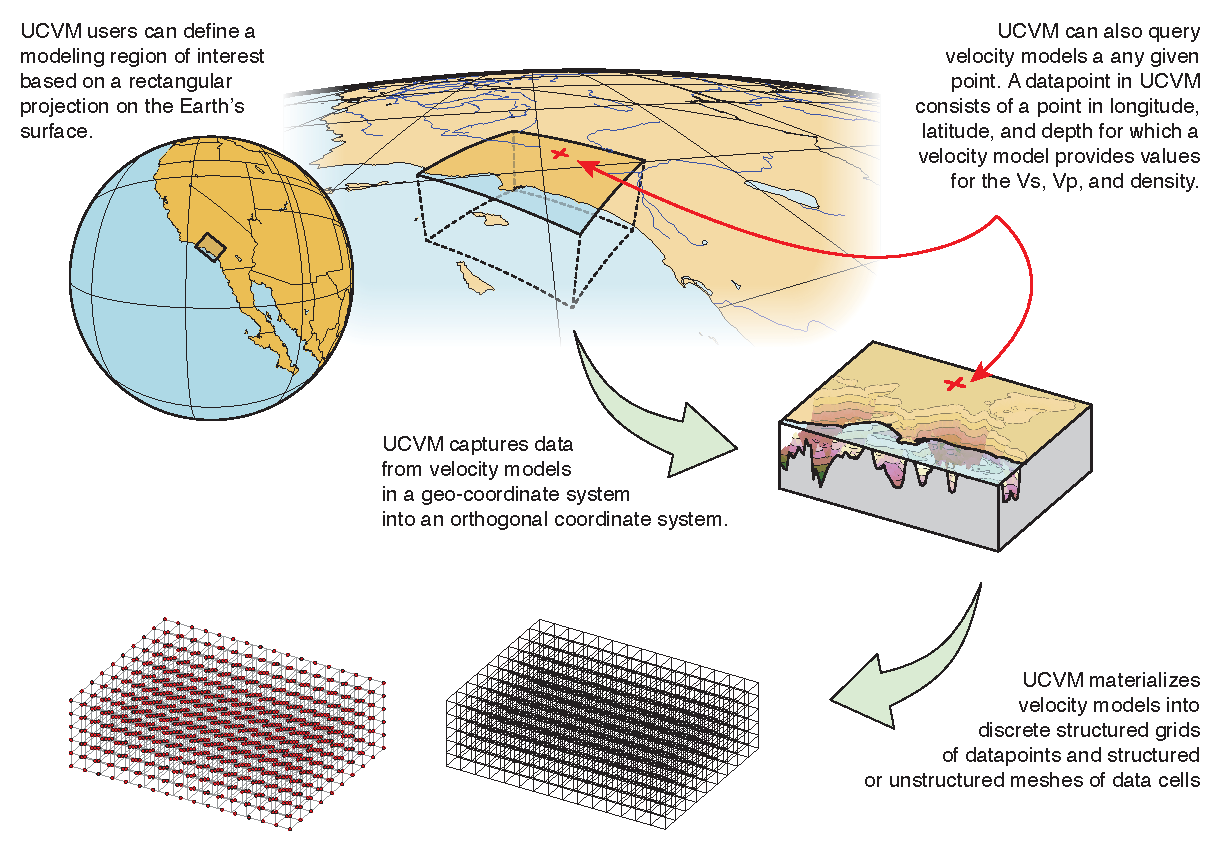
\includegraphics
		[width=0.9\textwidth]
		{figures/pdf/ucvm-model-extraction}
	\caption{High-level description of the UCVM framework functionality illustrating the selection of a region of interest for which a user can obtain datapoints using the UCVM utilities and create materialized models in the form of discrete three-dimensional grids or meshes.}
	\label{fig:framework}
\end{figure*}




\begin{figure*}[ht!]
	\centering
	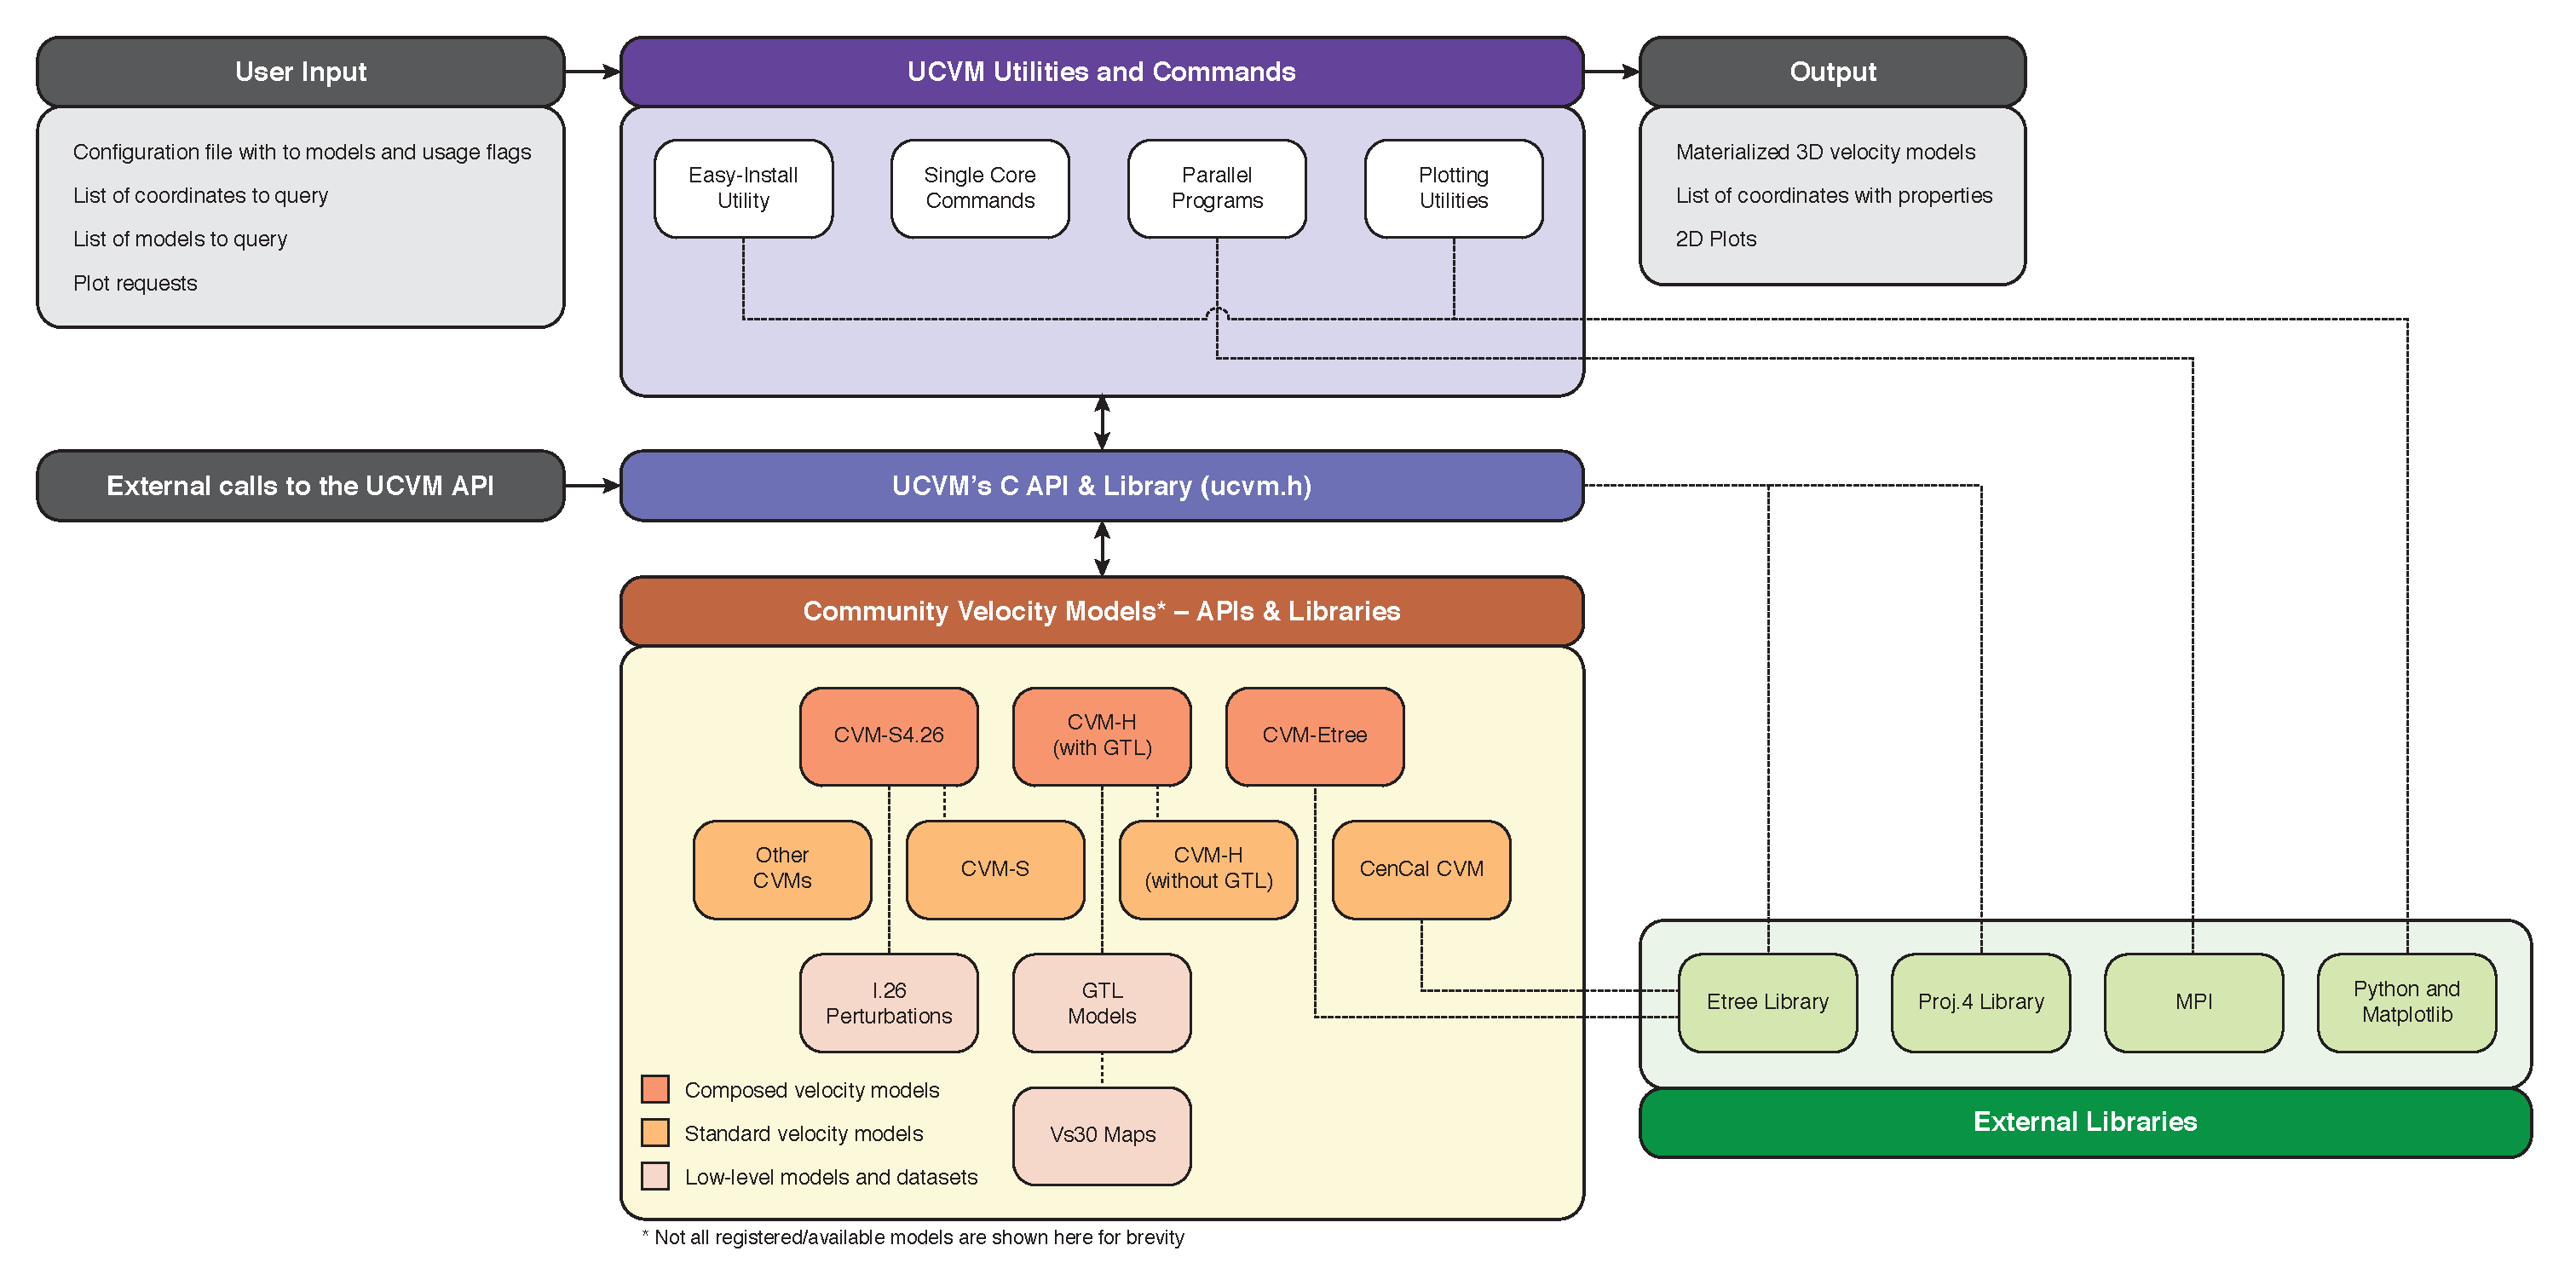
\includegraphics
		[width=\textwidth]
		{figures/pdf/ucvm-sw-architecture}
	\caption{The UCVM software architecture. Gray-colored frames indicate components at the level of user or client interaction. The upper purple-colored frame displays UCVM utilities and commands directly accessible to users, whereas the ligher purpled-colored box indicates the lower-level UCVM API and library upon which UCVM operations rest. Underlying this, are a selection of community models supported by UCVM; and to the right, in green, are the library dependencies of the UCVM framework. Here we distinguish models and datasets in four categories related to their origin or operational concept. In practice, however, UCVM treats each model or dataset independently and without any distinction.}
	\label{fig:sw.arch}
\end{figure*}



\begin{table*}[t]
\centering
\small
\caption{Electronic addresses to UCVM on-line documentation.}
\begin{tabular}[]{ll}
\\
Description                 & URL Address                                                         \\
\hline
General Documentation       & \url{http://scec.usc.edu/scecpedia/UCVM}                            \\
General User Guide          & \url{http://scec.usc.edu/scecpedia/UCVM_User_Guide}                 \\
Advanced User Guide 	    & \url{http://scec.usc.edu/scecpedia/UCVM_Advanced_User_Guide} 	  \\
Tutorial 	            & \url{http://scec.usc.edu/scecpedia/UCVM_Tutorial}            	  \\
Model Integration           & \url{http://scec.usc.edu/scecpedia/UCVM_Model_Integration_Guide}    \\
\hline
\end{tabular}
\label{tab:manuals}
\end{table*}


\section{The UCVM Software Framework}\label{sec:ucvm}

The primary functionality provided by UCVM is the ability to query a wide array of CVMs for material properties through a standardized query interface, and return material properties from the CVMs in standardized formats, independently of the particularities of each dataset or CVM. UCVM achieves this by registering datasets and velocity models into the framework. Registration of a velocity model or dataset consists of creating the appropriate API to facilitate the communication between the framework utilities and tools, and the velocity models and datasets. Once a velocity model or dataset has been registered with UCVM, a client can use the framework utilities to retrieve information from the models at any geographic point within the coverage region of the model(s). A client can be either a user (via the command-line) or a software application. The primary data type retrieved by a UCVM client for a single geographical point consists of a float triplet with the seismic velocities (\vp{} and \vs{}), and the material's density ($\rho$). At times we refer to this triple as the payload. The UCVM can then be used to produce standardized output in the form of three-dimensional (3D) volumetric datasets, two-dimensional (2D) vertical cross-sections and horizontal slices, and individual data points. This process is illustrated at a general level for the cases of 3D models in Figure \ref{fig:framework}. A client can also use other UCVM utilities for plotting and transforming models and datasets.

In order to facilitate access to the models, UCVM conceals each model's local coordinate system behind a generic querying interface. Data points are queried through this interface by geographic latitude and longitude, and a vertical $z$-coordinate. The framework allows defining the $z$-axis as either depth below the free surface (in meters, positive downward) or elevation relative to mean sea level (where zero is at sea level, positive upward and negative downward). The UCVM standardized interface allows multiple velocity models to be aggregated into a single composite model or meta-model. Composition is accomplished by tiling two or more velocity models in three dimensions according to a user-specified priority order. To support this flexible query mechanism consistently across all models, UCVM includes a high-resolution digital elevation model (DEM) and uses a cartographic projection library (Proj.4: \url{http://trac.osgeo.org/proj}). The DEM is synthesized from the USGS National Elevation Dataset \citep{Gesch_2002_PERS, Gesch_2007_Chap} and the ETOPO1 Global Relief Model \citep{Amante_2009_Manual}. The built-in DEM enables clients to retrieve the surface elevation at any query point in addition to the default data-point payload of material properties (\vp{}, \vs{}, $\rho$).

The abstraction of native CVM interfaces under a uniform API is illustrated by Figure \ref{fig:sw.arch}. This API is written in the C language, and may be invoked directly by an application program to query any registered model as described previously. Alternatively, the framework provides a small set of predefined command-line tools to perform common operations, such as querying points, creating meshes, and producing simple graphs. As these tools are themselves defined in terms of the API, they may be leveraged as templates for creating new utilities. This layered approach to the framework design allows for future extensibility both in terms of new model support, and querying functionality.

With the exception of the Wasatch Front (Utah) CVM, the primary focus area of UCVM has been on models available for the State of California (and portions of neighboring States). However, the framework has been designed to be easily modified to cover any arbitrary region of the Earth's surface, provided adequate resolution velocity and elevation models exist. Additional details about the models available through UCVM are given in the following section on Community Velocity Models. Subsequent sections provide further information on the main UCVM features. However, due to space limitations, not all utilities and options are described in detail here. For additional in-depth information, general and advanced users should refer to the on-line manuals and documentation. Table \ref{tab:manuals} provides URL addresses linking to permanent supporting material. The last section of the paper is dedicated to simple examples and recent case applications of UCVM. 

